\documentclass{article}

\usepackage[utf8]{inputenc}
\usepackage{url}
\usepackage{amsmath}
\def\UrlFont{\em}
\usepackage{indentfirst}

\title{Trabalho de Visão Relatório}
\author{Felipe Leivas Machado - 262528 \and Priscila Cavalli Rachevsky - 261573 }

\usepackage{natbib}
\usepackage{graphicx}
\usepackage{capt-of}

\begin{document}

\maketitle

\section{Introdução}
    A partir de uma imagem com linhas que representavam os eixos \(X\) e \(Y\) de um plano cartesiano e uma parábola precisava plotar essas linhas novamente, garantindo que os eixos eram perpendiculares e que a parábola seguisse uma equação de segundo grau. Para isso, precisou seguir esses passos:
   \begin{itemize}
       \item Extrair uma imagem de bordas
       \item Identificar os eixos \(X\) e \(Y\)
       \item Remover os eixos
       \item Forçar eixos perpendiculares
       \item Identificar a parábola
       \item Desenhar a parábola
   \end{itemize}
\section{Implementação}
   \subsection{Extrair uma imagem de bordas}
   Primeiramente, a imagem foi transformada para ter apenas tons cinza. Então, se aplicou o filtro Gaussiano com kernel tamanho 7 para diminuir eventuais ruídos. Dessa forma, aplicou-se binarização, no qual o linear tinha o valor de 143.
   \begin{figure}[h!]
   \centering
    \subfigure
        {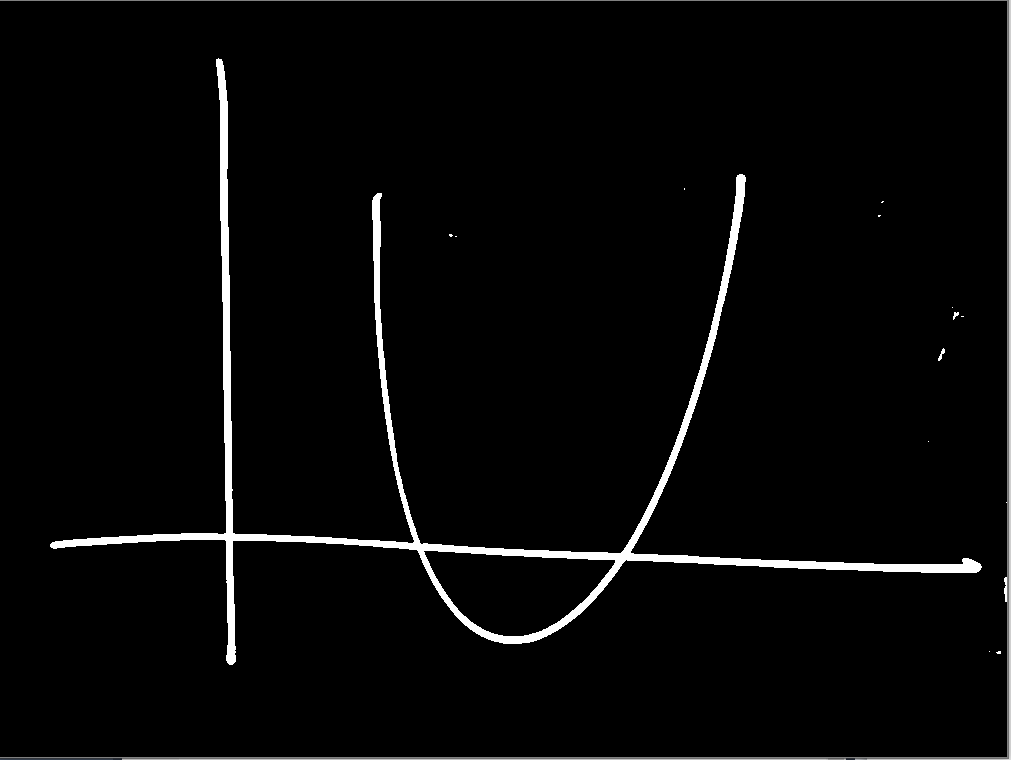
\includegraphics[scale=0.17]{exemplo1_edge.PNG}}
    \subfigure
        {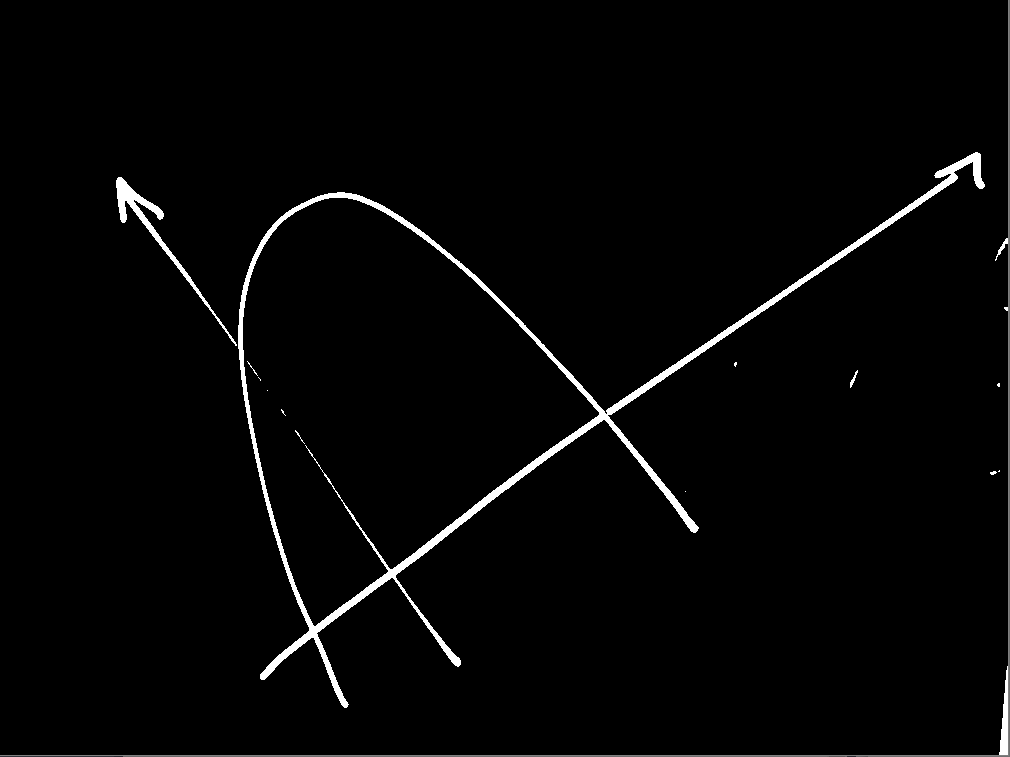
\includegraphics[scale=0.17]{exemplo2_edge.PNG}}
    \subfigure
        {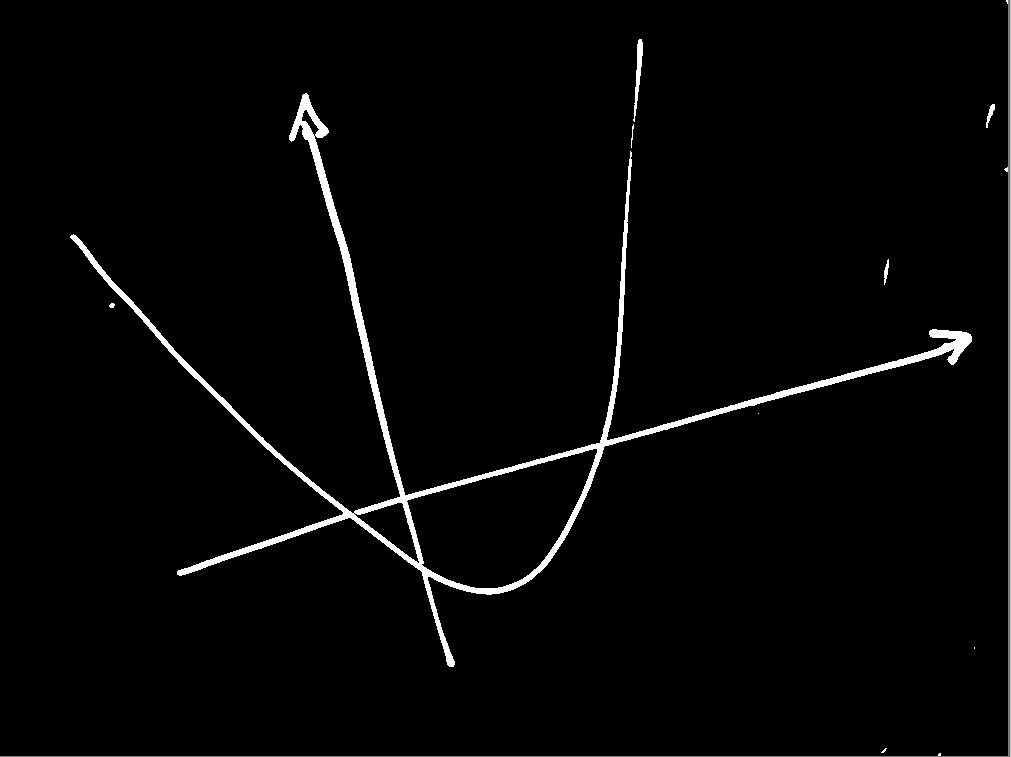
\includegraphics[scale=0.17]{exemplo3_edge.PNG}}
    \caption{Imagens de bordas}
    \end{figure}

   \subsection{Identificar os eixos \(X\) e \(Y\)}
   Usou-se Hough para identificar todas linhas que atendiam aos critérios de:
   \begin{itemize}
       \item    Tamanho mínimo de 300 pixels
       \item    Gap máximo de 50 de gap
   \end{itemize}


   Então, identificou-se que as linhas eram eixo \(X\) quando a diferença entre seus 2 pontos era maior no \(x\) do que no \(y\), ou seja, \((x_1 - x_2)^2 > (y_1 - y_2) ^2\), caso contrário, a linha representava o eixo \(Y\).

  Para determinar a reta do eixo \(X\), foi usado mínimos quadráticos em todas as linhas identificadas como eixo \(X\). Já para determinar o eixo \(Y\), se calculou mínimos quadráticos apenas para as linhas que estavam próximas a maior linha de todas que foram classificadas como eixo \(Y\), porque em alguns casos partes da parábola eram reconhecidas como sendo do eixo Y.

 \subsection{Forçar eixos perpendiculares}
   Com esses retas se determinou a origem do sistema. Para garantir que as duas fossem perpendiculares, recalculamos a reta \(Y\) a partir da reta \(X\), ou seja, foi pego a reta perpendicular à \(X\) e que passasse pela origem do sistema.

   \subsection{Remover os eixos}
   Simplesmente foram desenhadas duas linhas (eixos \(Y\) e \(X\)) pretas com 80 pixels de largura na imagem de borda. Dessa forma, a remoção foi feita com sucesso. Precisou de uma largura alta para remover também as setas dos eixos que haviam nos exemplos 2 e 3.
   \begin{figure}[h!]
   \centering
    \subfigure
        {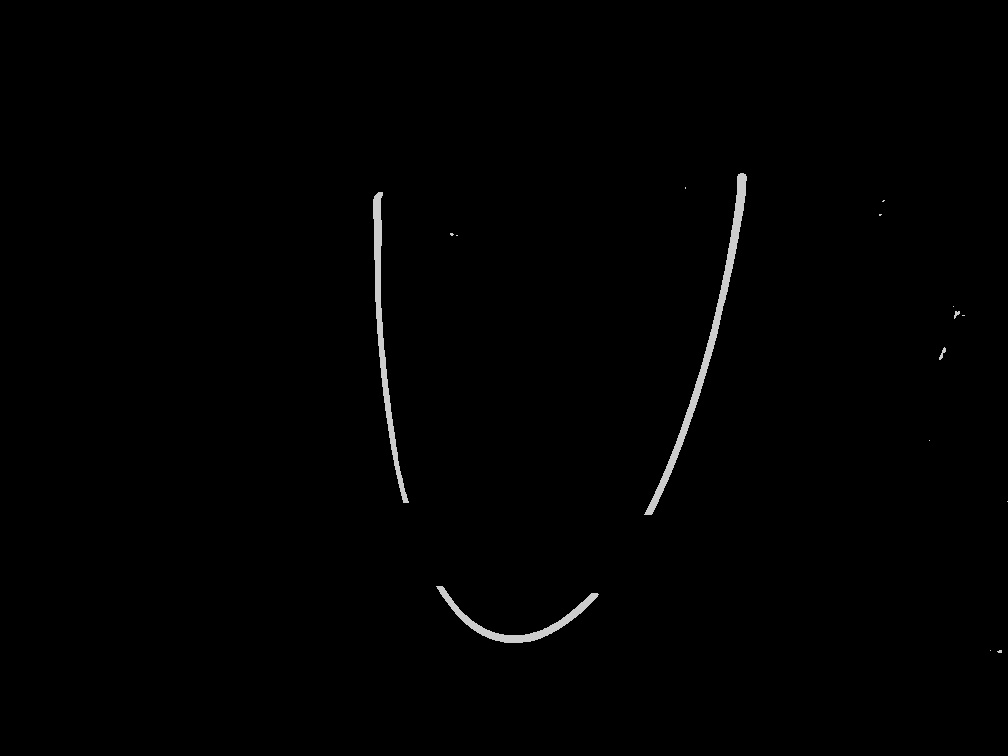
\includegraphics[scale=0.1]{exemplo1WithoutAxis.jpg}}
    \subfigure
        {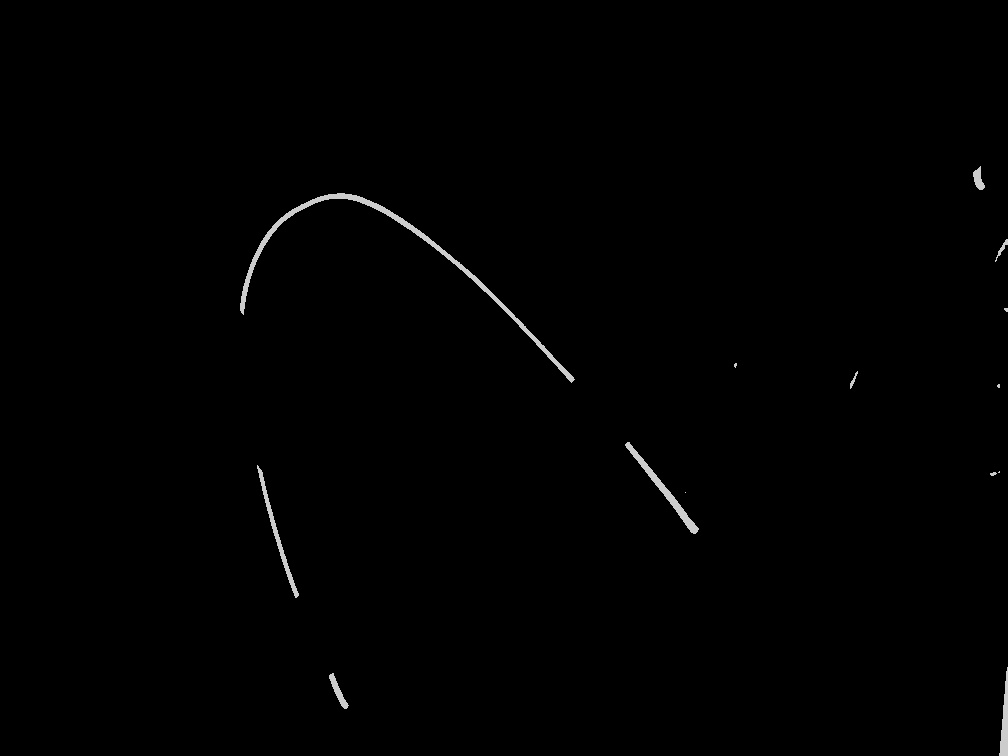
\includegraphics[scale=0.1]{exemplo2WithoutAxis.jpg}}
    \subfigure
        {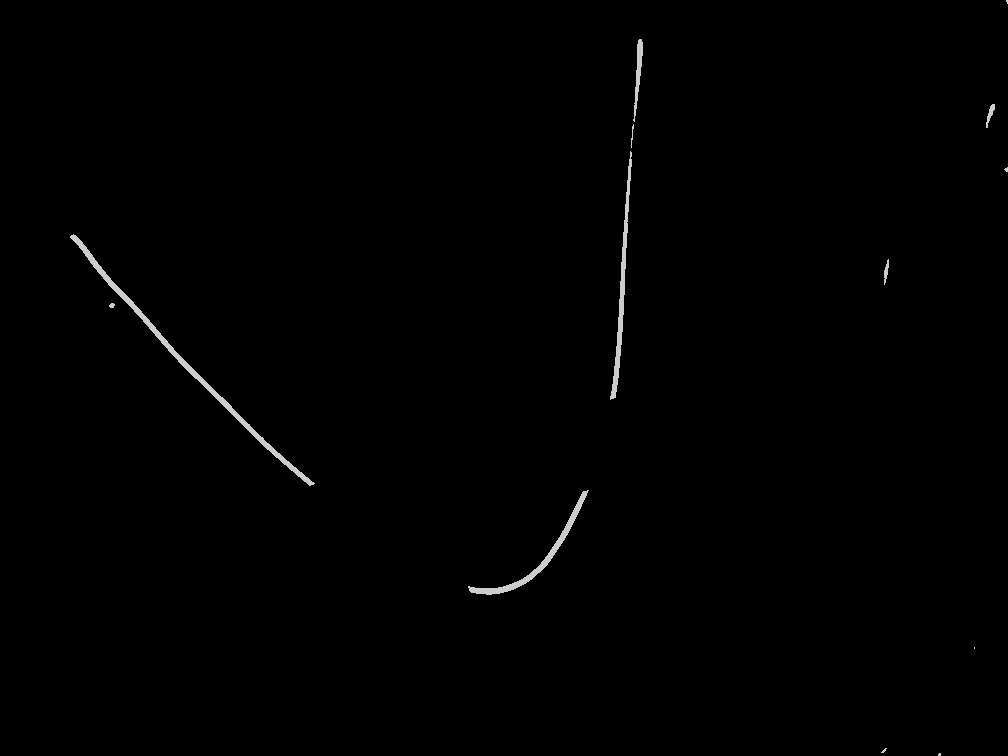
\includegraphics[scale=0.1]{exemplo3WithoutAxis.jpg}}
    \caption{Imagens após remoção dos eixos }
    \end{figure}

\subsection{Identificar a parábola}

    \subsubsection{Identificação dos pontos}
    Foi utilizado Hough para descobrir as linhas que restaram na imagem de borda, elas representariam os pontos da parábola.
    \subsubsection{Rotação dos pontos para o eixo \(XY\)}
    Usando a reta do eixo \(X\) como base, pegou o ângulo de inclinação dela, e todos pontos foram rotacionados para o eixo \(XY\), utilizando a matriz de rotação.
    \subsubsection{Cálculo da parábola}
    Utilizando mínimos quadráticos com todos os pontos identificados, se descobriu a reta que passava por eles e que se encaixava na formulação \(ax^2 + bx + c = y\). Assim, as equações encontradas foram:
   \begin{itemize}
       \item Exemplo 1:  \(0.0128x^2 -14.3060x+3379.4024\)
       \item Exemplo 2: \(-0.0094x^2+0.8472x-370.6317\)
       \item Exemplo3:  \(0.0054x^2-3.3020x-190.7882\)
   \end{itemize}




\subsection{Desenhar a parábola}

Se calculou os pontos de acordo com a equação da parábola e os rotacionou sentido contrário a sessão anterior, dessa forma, o ponto que estava no plano cartesiano foi encontrado no plano da imagem. Então, se desenhou um circulo para cada ponto, como eram muito próximos, representou a reta da parábola perfeitamente.

\begin{figure}[h!]
   \centering
    \subfigure
        {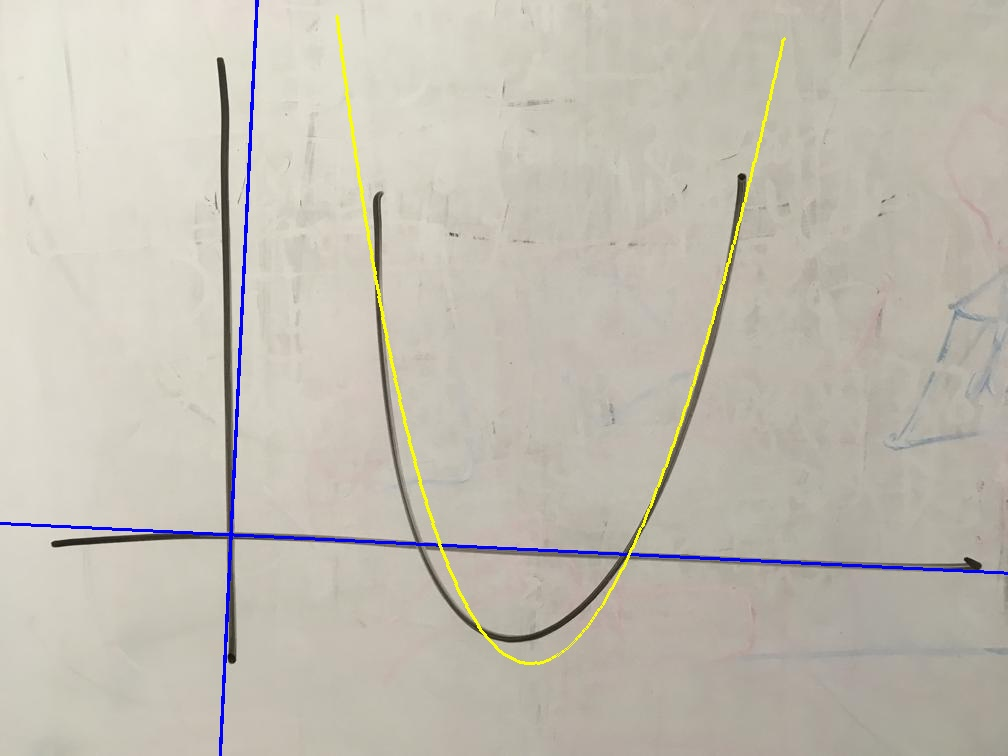
\includegraphics[scale=0.2]{exemplo1ParaboleImage.jpg}}
    \subfigure
        {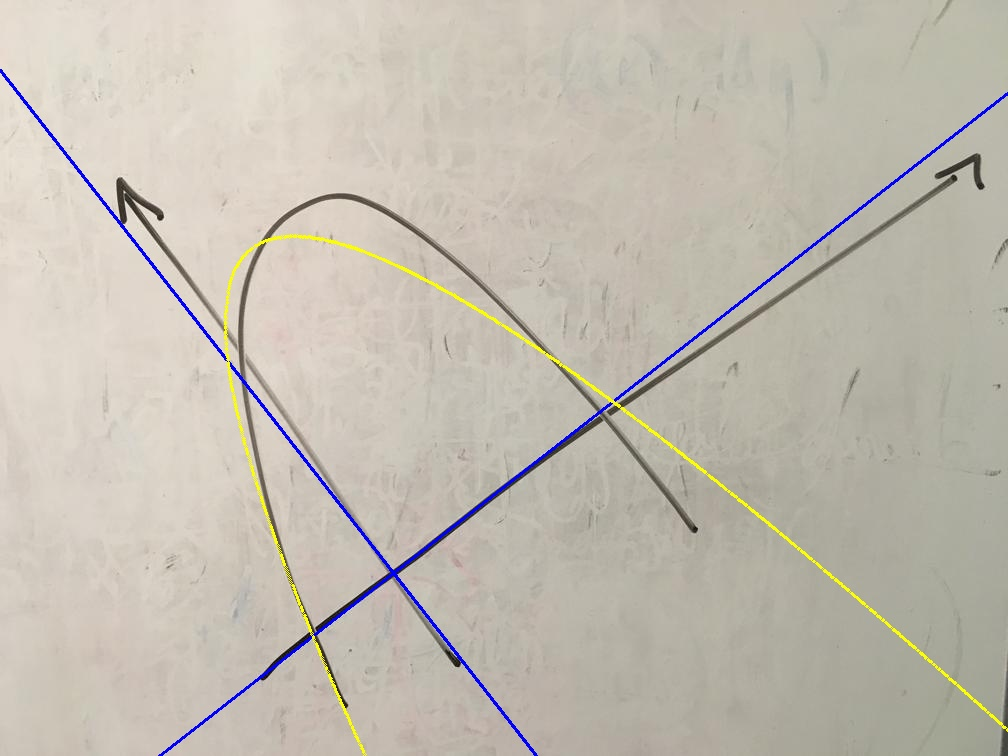
\includegraphics[scale=0.2]{exemplo2ParaboleImage.jpg}}
    \subfigure
        {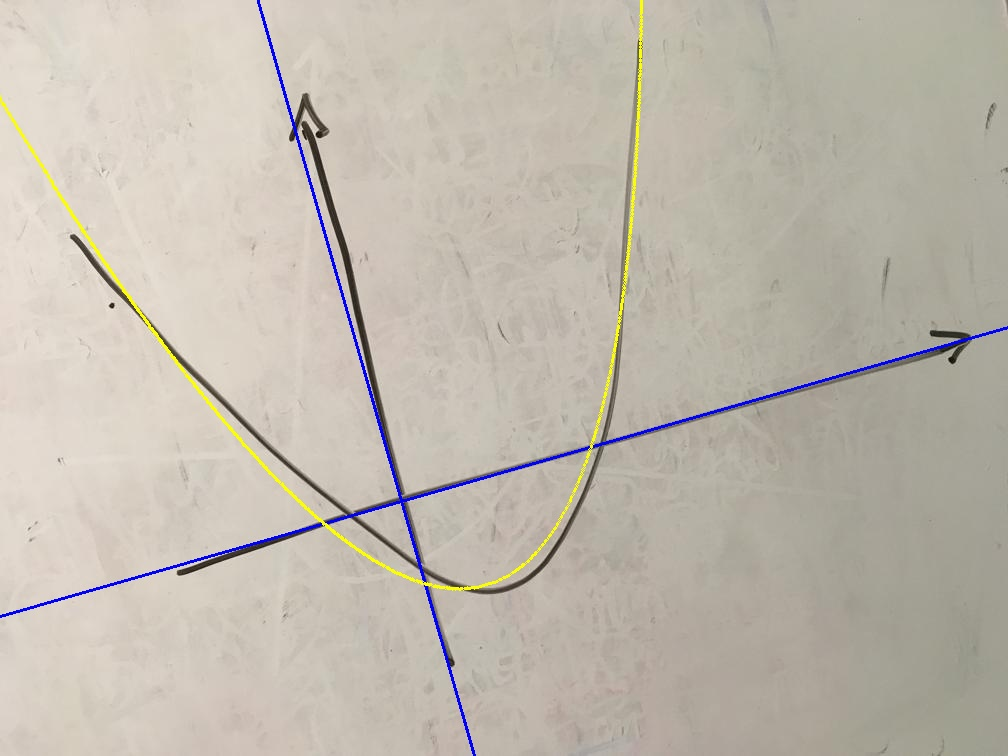
\includegraphics[scale=0.2]{exemplo3ParaboleImage.jpg}}
    \caption{Resultado do trabalho }
\end{figure}
    
    % \[
    % A = 
    %     \begin{bmatrix}
    %     x_1^2   & x_1 & 1 \\
    %     x_2^2   & x_2 & 1 \\
    %     \hdotsfor{3} \\
    %     x_n^2   & x_n & 1 \\
    %     \end{bmatrix}
    % B = 
    %     \begin{bmatrix}
    %     y_1 \\
    %     y_2 \\
    %     \hdotsfor{1} \\
    %     y_n \\
    %     \end{bmatrix}
    % X = 
    %     \begin{bmatrix}
    %     a &  b & c
    %     \end{bmatrix}
    % \]
    
    % \(    A ^ T * A * X = A ^ T * B \)
\end{document}
